\documentclass{scrartcl}

\usepackage[T1]{fontenc}
\usepackage[utf8]{inputenc}

\title{Mobile Dev Week 3 Lab}
\author{Daniel Coady (102084174)}
\date{02/09/2019}

\usepackage{graphicx}

\begin{document}

\maketitle

\section*{Food Parcels}
\subsection*{Task 1}
\begin{figure}[h]
    \centering
    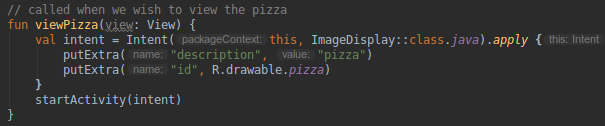
\includegraphics[scale=0.6]{images/screen1.png}
    \caption{The code that allows the  two activities to connect with each other}
\end{figure}

To allow for each activity to communicate with each other for consistency across the app,
we can use intents. With intents we are able to declare what activity we wish to be able to
move onto as well as the data that should go along with it. In this case we are able to send
a description and the id of the photo that has been touched so that we can show a larger version
of it along with it's short description.

\pagebreak

\begin{figure}[h]
    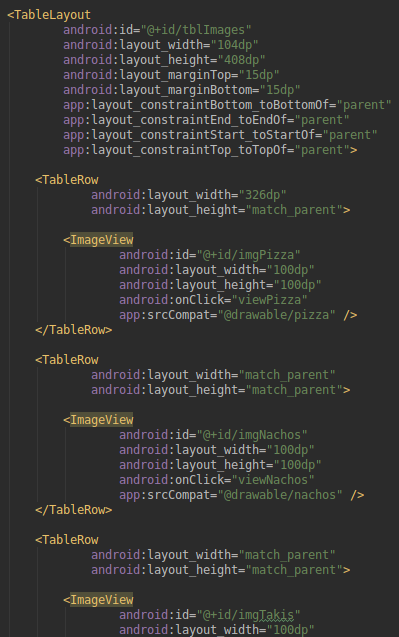
\includegraphics[scale=0.4]{images/screen2.png}
    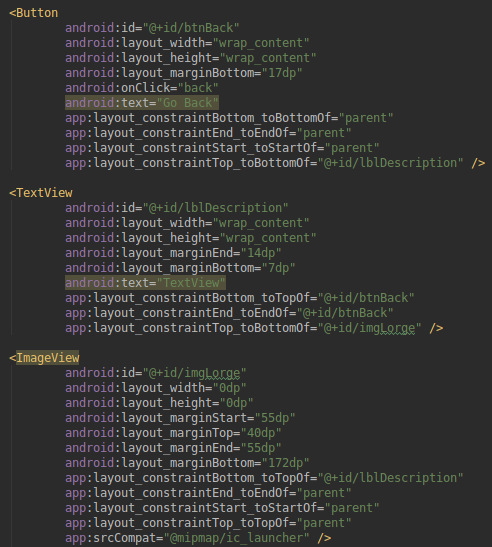
\includegraphics[scale=0.4]{images/screen3.png}
    \caption{Part of the XML used for the activities}
\end{figure}

\pagebreak

\begin{figure}[h]
    \centering
    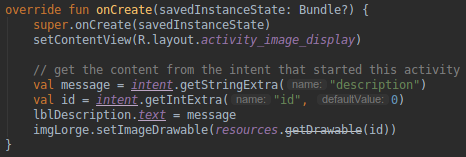
\includegraphics[scale=0.6]{images/screen4.png}
    \caption{Code used to set the views in the image view activity}
\end{figure}

Here we are now collecting the information stored in the intent from the previous activity to
display the information requested.

\pagebreak

\begin{figure}[h]
    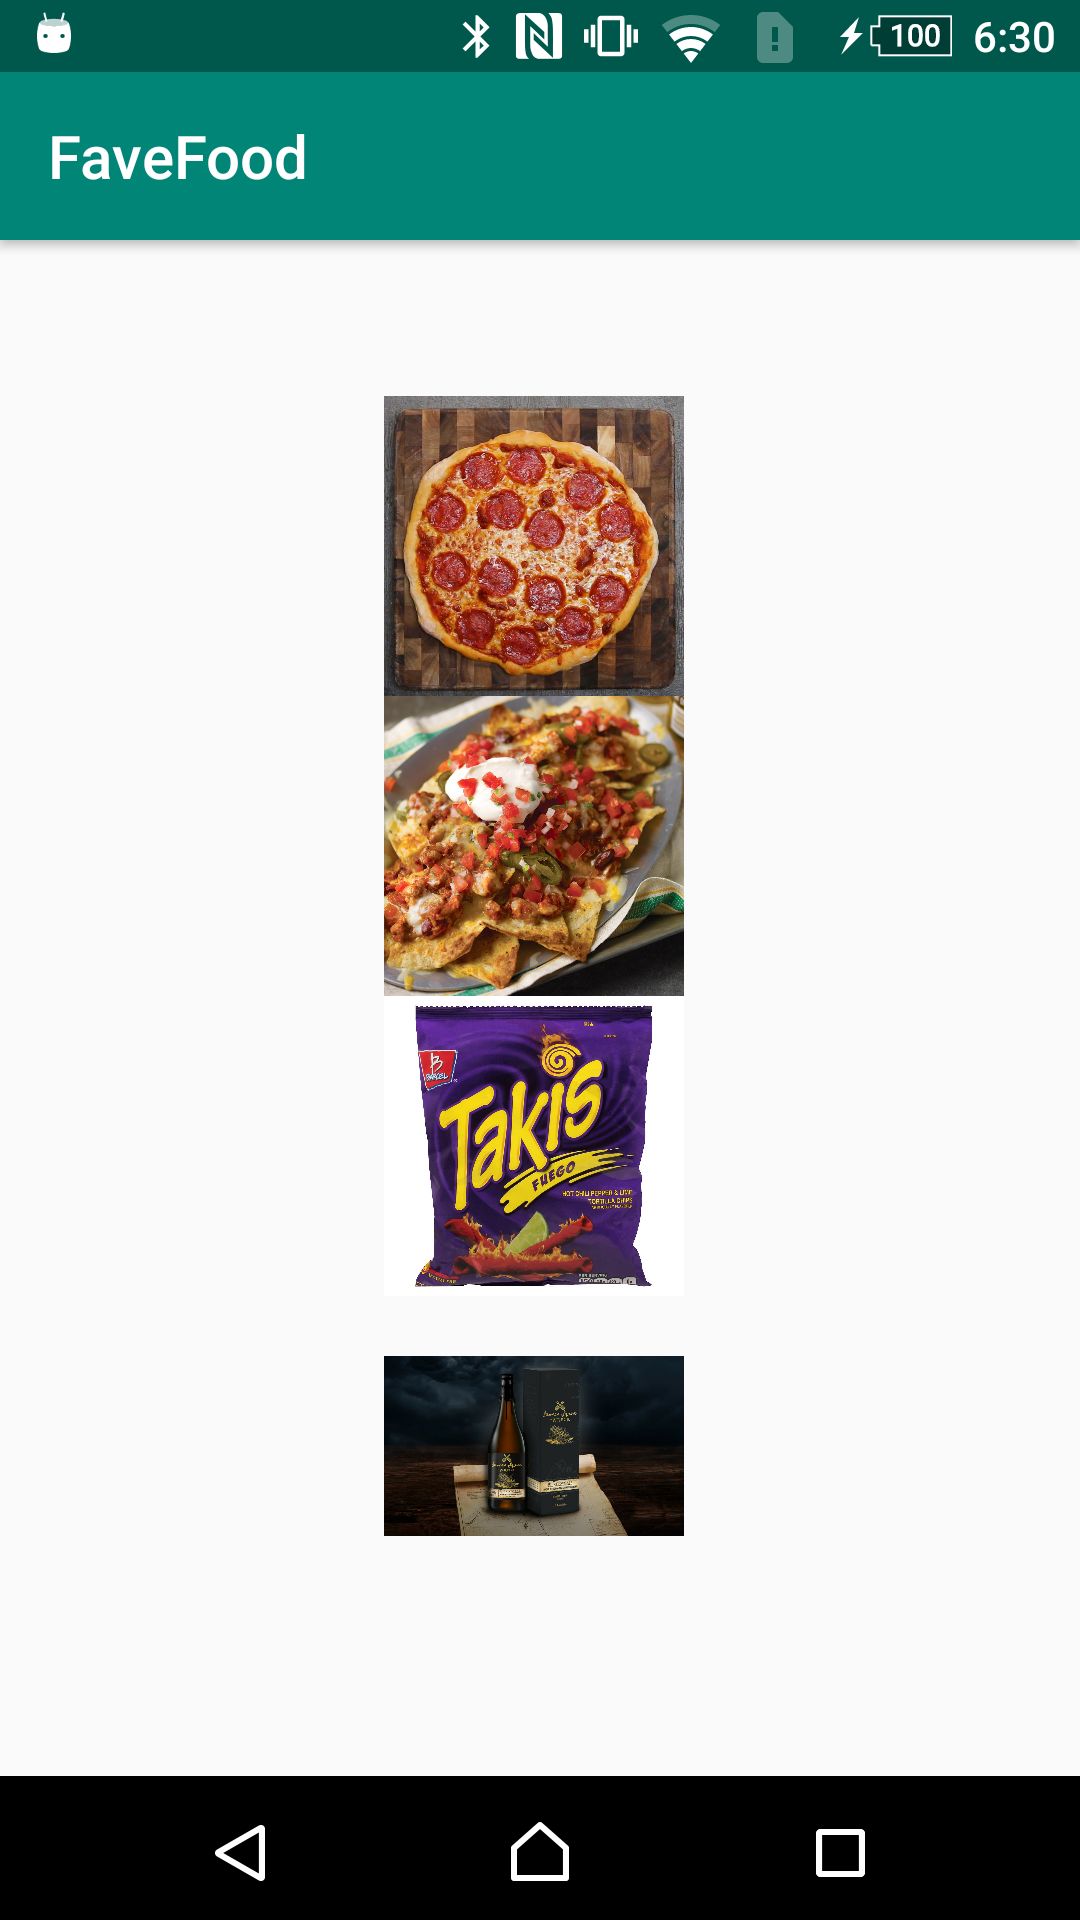
\includegraphics[scale=0.15]{images/screen5.png}
    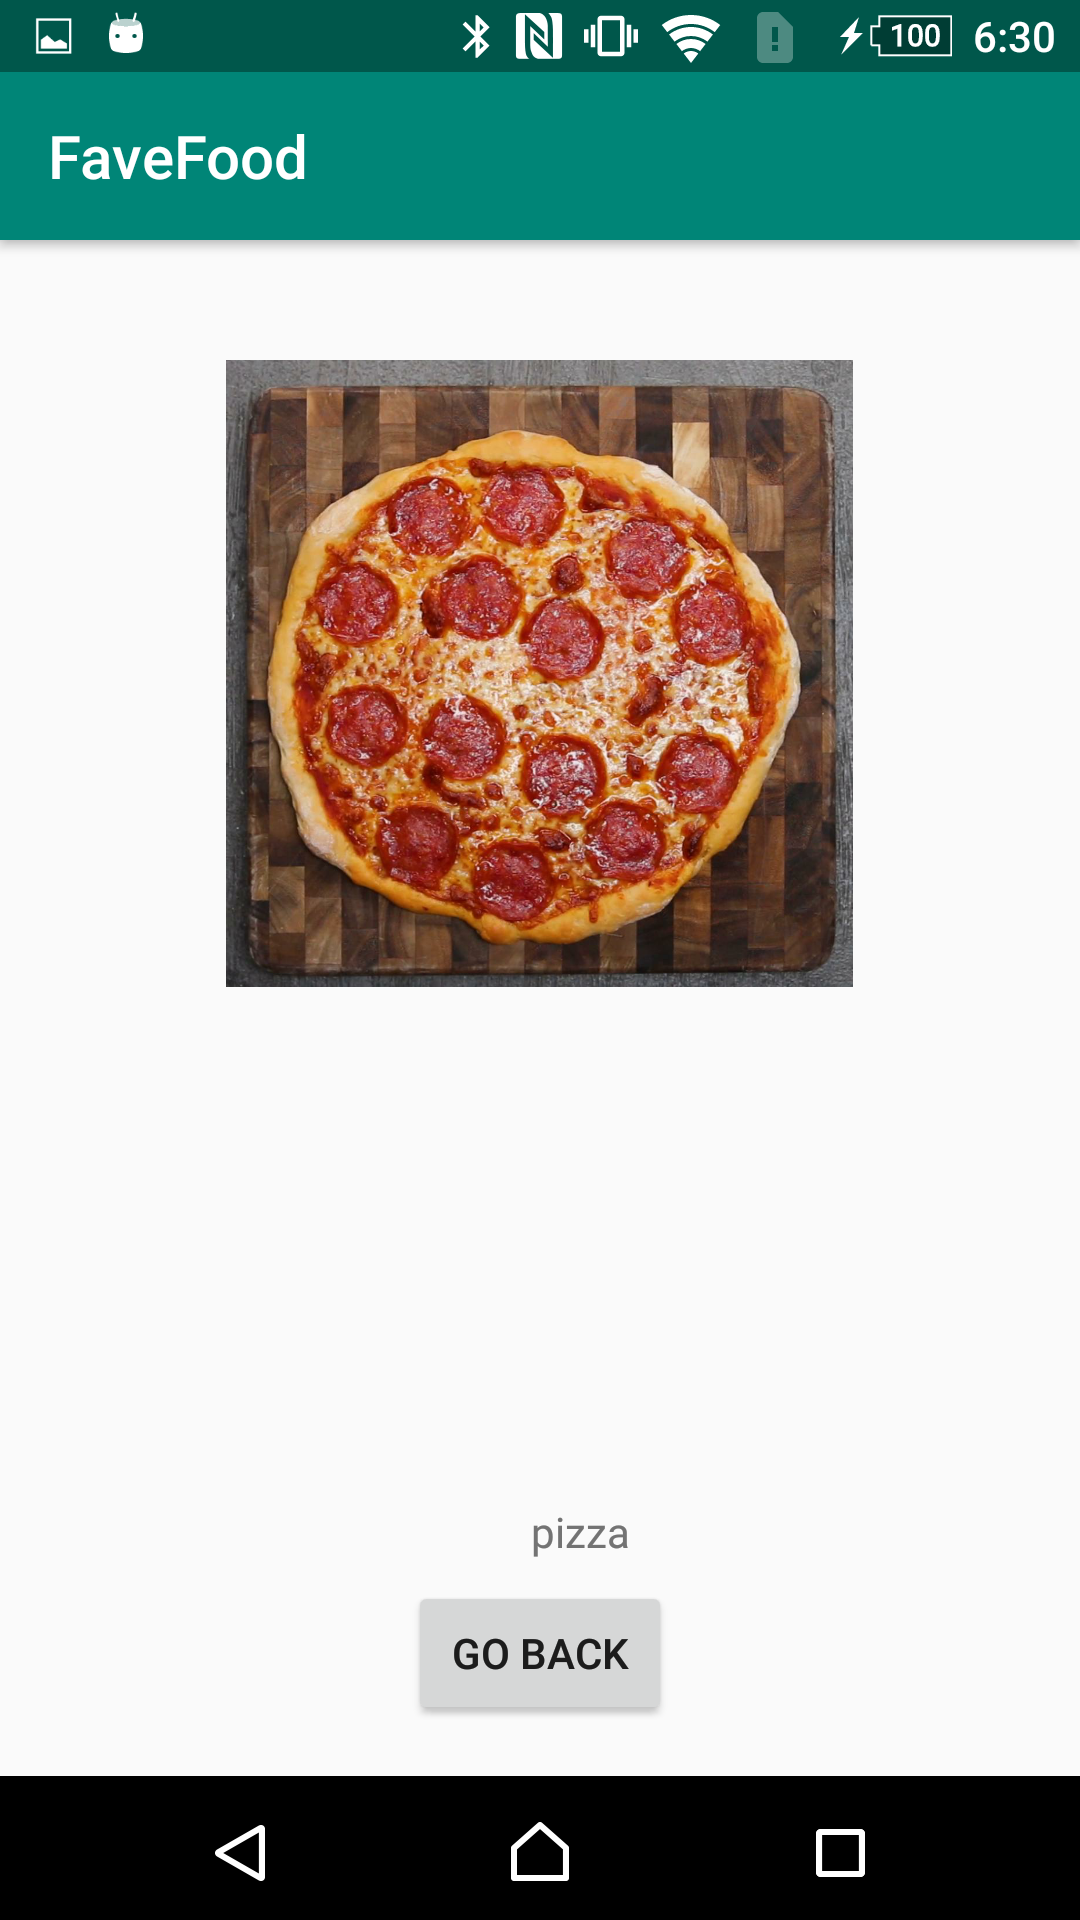
\includegraphics[scale=0.15]{images/screen6.png}
    \caption{The application in action}
\end{figure}

\pagebreak

\subsection*{Task 2}
For this task we have expanded upon the idea of the first task by creating sets of metadata for each
of the images that we are then able to edit once we inspect a photo.

\begin{figure}[h]
    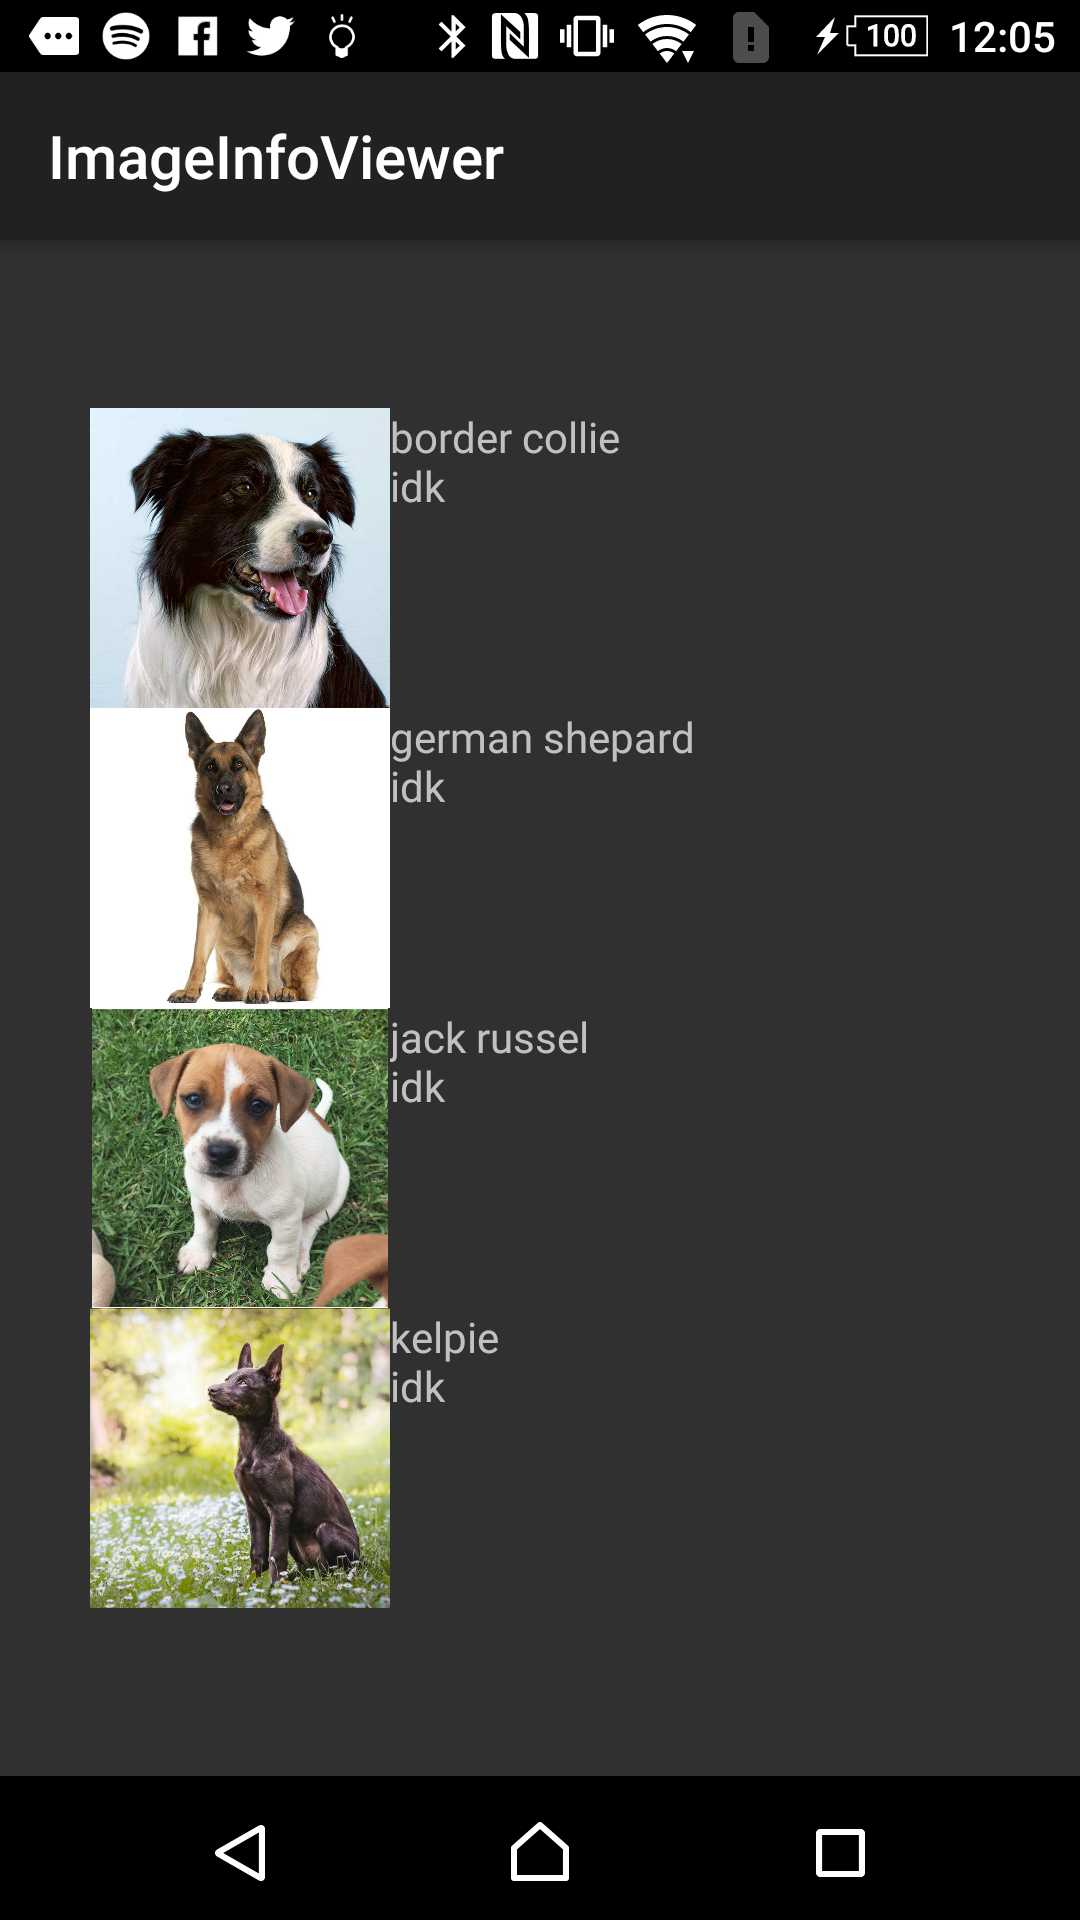
\includegraphics[scale=0.15]{images/screen7.png}
    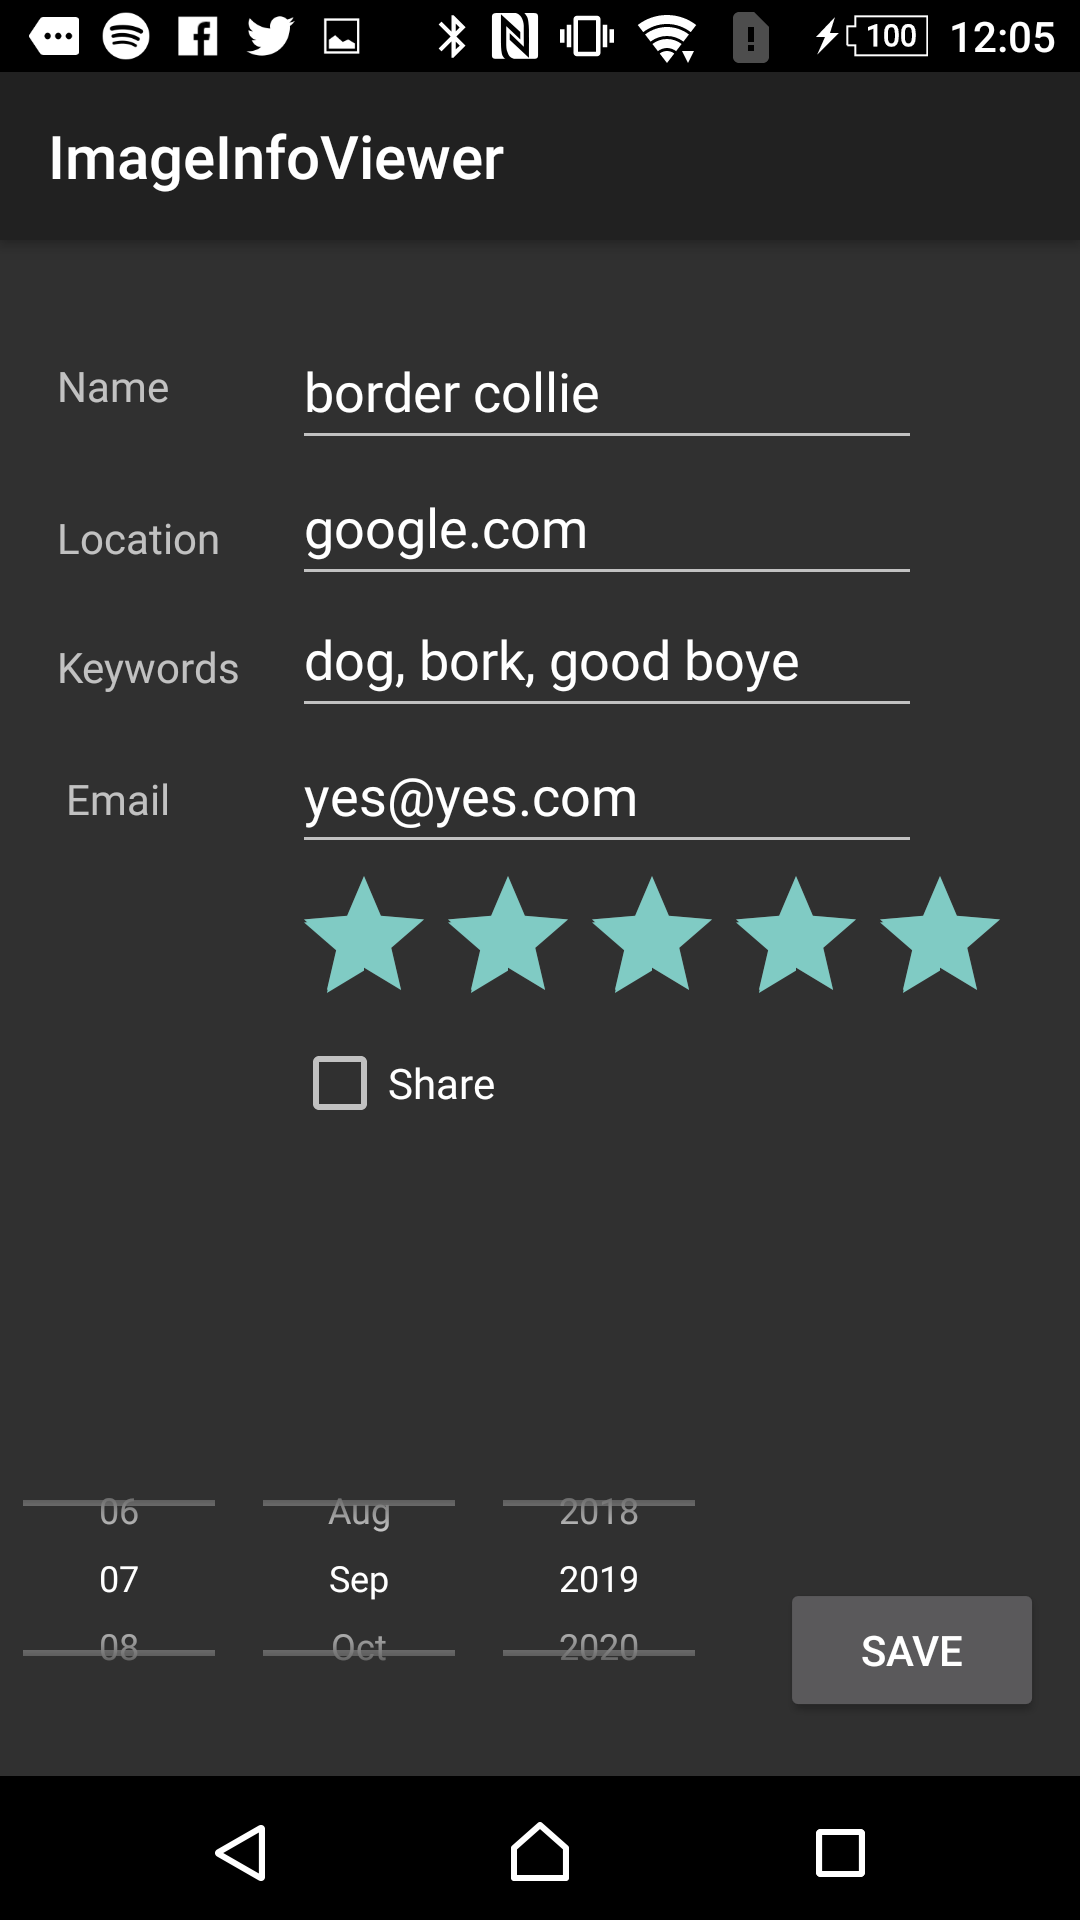
\includegraphics[scale=0.15]{images/screen8.png}
    \caption{The two activities used for the task}
\end{figure}

To achieve the dark theme that is present in borht activites, I had to edit the AndroidManifest.xml
file which is where many global settings for the application are stored. In this case we just need
to edit the android:theme line te equal @style/Theme.AppCompat and then everything else would be
handled for us.

\begin{figure}[h]
    \centering
    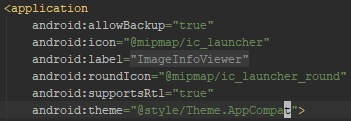
\includegraphics{images/styles.jpg}
    \caption{Part of the file AndroidManifest.xml}
\end{figure}

\pagebreak

The other key part of this task was the use of the parcelable interface to allow for sending of
data classes between two activities. The parcelable interface is used to allow classes that contain
primitive types to be sent across activities using intents. Through the magic of polymorphism, we
are able to implement this interface into our classes to enable them to be accepted as arguments when
being added as an extra to an intent. From there, you are able to then access them as normal within
the other activity.

\begin{figure}[h]
    \centering
    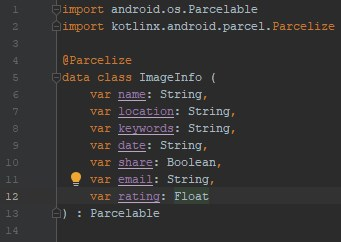
\includegraphics{images/parcelableclass.jpg}
    \caption{The data class used in this task, which implements the parcelable interface}
\end{figure}

\end{document}
